\documentclass{article}
\usepackage{amsmath}
\usepackage{hyperref}
\usepackage{graphicx}
\usepackage{booktabs}
\usepackage{float}
\hypersetup{
	colorlinks=true,
	linkcolor=blue,
	filecolor=magenta,      
	urlcolor=blue,
	pdfpagemode=FullScreen,
}
\usepackage{natbib}
\bibliographystyle{plainnat}

\begin{document}


\section{Abstract}	
The aim of this document is to document the recreation of the CSTR model defined in \cite{pilario2018canonical}. This document goes hand-in-hand with the IPython notebook 
"CSTR Model Python" which uses the methodology specified here to generate the CSTR data set in the Python programming language. The end result was compared against the results presented by \cite{pilario2018canonical} with reasonable success for normal operation. The code can be freely used to generate normal and incipient fault data sets as a way of testing fault detection models. Furthermore, the code can also be used to generate other data sets that might be of interest for use in further study.


\section{Introduction}

\cite{pilario2018canonical} developed a model for the detection of incipient faults. To test their model, they developed a simulation model of a CSTR that was modified to take into account the intricacies of real-time data. This includes things such as parameter mismatch, sensor drift, Gaussian noise and other phenomena that cause a process to deviate from theoretically ideal behaviour. The benefit in doing this is that they can successfully test their fault detection model against normal behaviour and scenarios where a fault has been introduced. The aim of the fault detection model is naturally to minimize the occurrence of false positives in normal behaviour and minimize the lag in detection during faulty scenarios. 

The CSTR model in this paper was modelled in Simulink which is freely available \href{https://uk.mathworks.com/matlabcentral/fileexchange/66189-feedback-controlled-cstr-process-for-fault-simulation}{online} and can be subsequently used for data set generation for anyone with a MATLAB/Simulink license. However, in the interests of making this model and its resulting data set even more widely available, this document outlines how the CSTR model can be recreated with open source tools (in this case the Python programming language).

Furthermore, it is good scientific practice to replicate the results presented in academic literature as a way of encouraging transparency and reproducibility in research. To this end, a model has been created that seeks to replicate the results presented in \cite{pilario2018canonical} using the exact same constants and initial conditions. The model can then be subsequently used to create any data sets that are useful also for studies outside fault detection.


\section{Methodology}

\subsection{Process Overview}
\label{sec:process_overview}
We start with a model schematic of the physical process (shown in Figure \ref{fig1}) and the differential equations that describe its dynamics. The schematic shows a simple jacketed CSTR where a temperature controller is used to control the amount of cooling water that is required.
 
\begin{figure}[H]	\centering
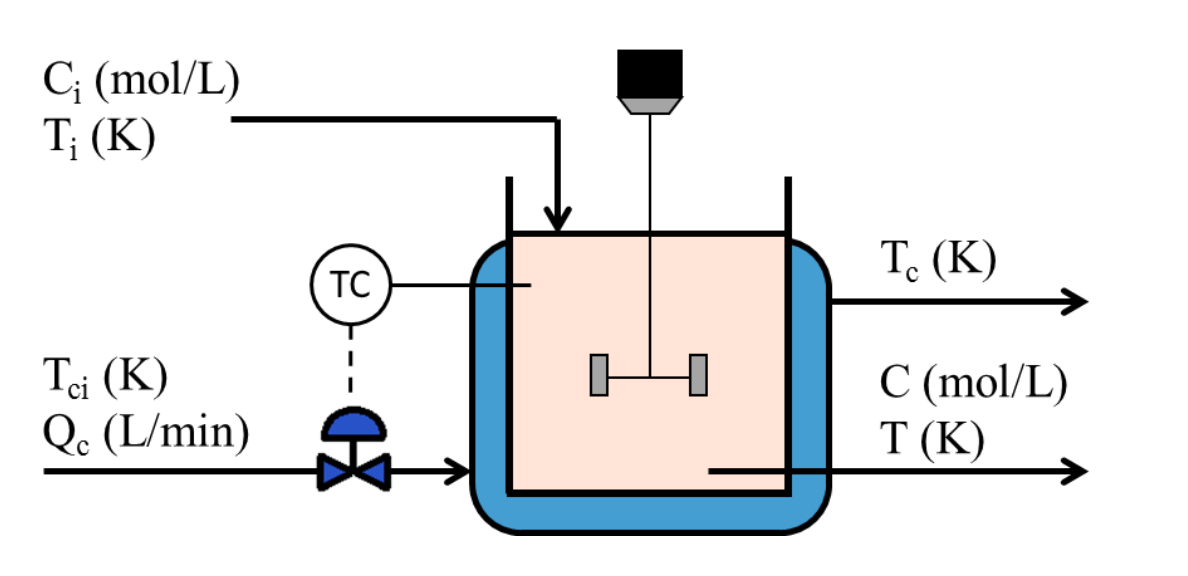
\includegraphics[width=\textwidth]{img/CSTR_schematic.png}
\caption{Schematic of a CSTR model taken from \cite{pilario2018canonical}}
\label{fig1}
\end{figure}

The inlet feeds in a concentration of reactant ($C_i$) some of which is transformed into a product that is not tracked. Thus the total component balance can be written as the following (assuming that the flow rate $Q$ and volume $V$ doesn't change with time): 

\begin{equation}
	\frac{dC}{dt} = Q/V(C-C_i)-kC
\end{equation} 

where $k$ is the reaction constant controlling the conversion of the reactant. The reaction is assumed to be an exothermic 1st order reaction that follows the Arrhenius equation for its reaction coefficients:

\begin{equation}
	k = k_0 e^{-E_a/RT}
\end{equation}

where $E_a$ is the activation energy, $R$ is the universal gas constant , $T$ is the temperature of the reactor and $k_0$ is a constant.The energy balance for the production takes into account the amount of energy entering and leaving the system in the production stream, as well as the heat generated by the exothermic reaction and the heat removed with the cooling jacket. The equation can be written as:

\begin{equation}
	\frac{dT}{dt} = (T_i-T)\frac{Q C_p}{V}+\frac{kC\Delta H_{r}}{\rho C_p}-\frac{UA(T-T_c)}{\rho C_p V}
\end{equation}

where $T_i$ is the inlet temperature, $C_p$ is the heat capacity of the fluid in the reactor, $\Delta H_r$ is the rate of heat given out by the reaction, $T_ci$ and $T_c$ is the inlet and exit temperature of the cooling water, $Q_c$ is the flow rate of the cooling water, $V_c$ is the volume of the cooling jacket and $C_{pc}$ is the heat capacity of the cooling water. The energy balance for the cooling jacket is 
\begin{equation}
	\frac{dT_c}{dt} = (T_{ci}-T_{c})\frac{Q_c}{V_c} +\frac{UA(T-T_c)}{\rho_c C_{pc} V_c	} 
\end{equation}

The rate of cooling water itself is controlled by the cooling water valve which strives to reach a temperature setpoint. This was implemented using a PI controller. 

\begin{equation}
	Q_c = Q_{c, 0} + K_p(T-T_{sp}) + \frac{1}{\tau_i}\int_{0}^{T}(T-T_{sp})dt 
\end{equation}
where $K_p$ is the proportional controller gain, $\tau_i$ is the integral time, $T_{sp}$ is the temperature set point and $Q_{c, 0}$ is the controller bias which represents the last value of the controller variable when the controller was turned from manual to auto.

\subsection{Constants and Inlet Conditions}
\label{sec:parameters}

The reactor, reaction, fluid and controller constants are given in Table \ref{tab:reactor_conditions}, Table \ref{tab:reaction_constants}, Table \ref{tab:fluid_constants} and Table \ref{tab:controller_constants}.

\begin{table}[h]
	\caption{Reactor parameters}
	\label{tab:reactor_conditions}
	\centering
	\begin{tabular}{lrl}
		\toprule
		{} &  Value &  Units \\
		Tags &        &        \\
		\midrule
		$V$  &      150 &  L \\
		$V_c$  &    10 &      L \\
		$UA$  &    7E5 &      cal/min/K \\
		$Q$  &    100	 &      L/min\\
		\bottomrule
	\end{tabular}
\end{table}


\begin{table}[H]
	\caption{Reaction constants}
	\label{tab:reaction_constants}
	\centering
	\begin{tabular}{lrl}
		\toprule
		{} &  Value &  Units \\
		Tags &        &        \\
		\midrule
		$E_a$  &      83,140 &  J/mol \\
		$R$  &    8.314 &   J/K/mol \\
		$\Delta H_r$  &    -2E5 &      cal/mol \\		
		$k_0$  &    7.2E10	 &      1/min \\
		\bottomrule
	\end{tabular}
\end{table}



\begin{table}[H]
	\caption{Fluid constants}
	\label{tab:fluid_constants}
	\centering
	\begin{tabular}{lrl}
		\toprule
		{} &  Value &  Units \\
		Tags &        &        \\
		\midrule
		$C_p$  &     1 &  cal/g/k \\
		$\rho$  &     1000 &  g/L \\
		$C_{pc}$  &    1 &   cal/g/k \\
		$\rho_c$  &     1000 &  g/L \\
	\end{tabular}
\end{table}



\begin{table}[H]
	\caption{Controller constants}
	\label{tab:controller_constants}
	\centering
	\begin{tabular}{lrl}
		\toprule
		{} &  Value &  Units \\
		Tags &        &        \\
		\midrule
		$K_c$  &     1 &  - \\
		$\tau_i$  &    0.2 &   1/min \\
		$T_{sp}$  &    430 &   K \\
	\end{tabular}
\end{table}

The initial conditions are required for solving the differential equations. These can change between different simulations but for the purposes of this study they are given in Table \ref{tab:intial_conditions} below.

 

\begin{table}[H]
	\caption{Initial Conditions}
	\label{tab:intial_conditions}
	\centering
	\begin{tabular}{lrl}
		\toprule
		{} &  Value &  Units \\
		Tags &        &        \\
		\midrule
		$T$  &     440 &  K \\
		$C$  &    1 &   mol/L \\
		$T_c$  &    410 &   K \\
		$Q_c$  &    150 &   L/min \\
	\end{tabular}
\end{table}

The inlet conditions in the paper change over time ever 60 minutes to mimic real process behaviour. To compare the results in the paper with our own model, we look at the first 4 perturbations that happen before a fault is introduced at 200 min (so at 0 min, 60 min, 120 min and 180 min). These inlet conditions are given in Figure \ref{inlet_conditions_closeup} and are summarised in Table \ref{tab:inlet_conditions}.

\begin{figure}[H]
	\centering
	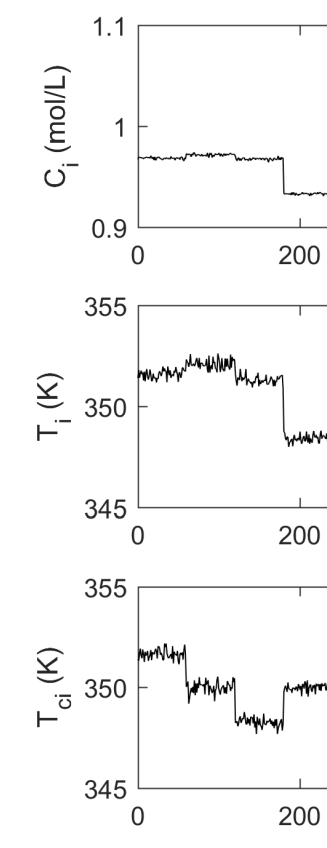
\includegraphics[width=0.25\textwidth]{img/inlet_conditions_closeup}
	\caption{Close up on initial conditions from \cite{pilario2018canonical}}
	\label{inlet_conditions_closeup}
\end{figure}


\begin{table}[H]
	\caption{Inlet conditions at 0, 60, 120 and 180 mins}
	\label{tab:inlet_conditions}
	\centering
	\begin{tabular}{lrl}
		\toprule
		{} &  Value &  Units \\
		Tags &        &        \\
		\midrule
		$C_i$  &      0.97, 0.97, 0.97, 0.93 &  mol/L \\
		$T_i$  &    351.5, 352.1, 351.2, 348.3
	 &      K \\
		$T_{ci}$ &    351.6, 349.8, 348.3, 349.8 &      K \\
		$Q$ &    100 &      L/min \\
		\bottomrule
	\end{tabular}
\end{table}


\subsection{Baseline Model}
\label{sec:baseline_model}

The best that we can do to compare a baseline steady model is to follow the results in Figure \ref{fig:results_paper_closeup} below. As expected, the variables $C$, $T$ and $T_c$ show only very minor changes over time. A notable exception is the cooling water flowrate $Q_c$ which sees a rapid drop from 150 L/min to 100 L/min for the conditions at 120 mins. As an estimate for the other variables, we guess that the values are around 0.1 mol/L, 430 K and 415 K for the concentration, reaction temperature and cooling jacket temperature respectively.  


\begin{figure}[H]
	\centering
	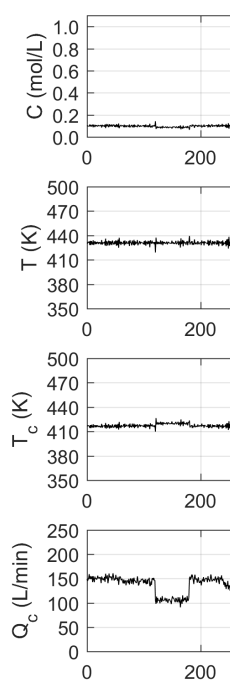
\includegraphics[width=0.25\textwidth]{img/results_paper_closeup}
	\caption{Close up of results from \cite{pilario2018canonical}}
	\label{fig:results_paper_closeup}
\end{figure}

\subsection{Simulation Procedure}


The differential equations were solved the "solve\_ivp" method from "scipy" using the Runge-Kutta ("RK45") method. A maximum step size of 0.01 minutes was used to help with solver convergence. The PI controller followed standard implementation re implementation. It was set to update the controller value only after an elapsed dt of 0.01 minutes and contains anti-reset windup to avoid integration issues when reaching controller saturation. The model for the baseline case was run for 20 minutes.

\subsection{Dataset Generation}

To generate "process data" from this model, a few things can be done to make it look real. This includes the following:

\begin{itemize}
	\item Dynamic perturbation of the inlet values of $C_i$, $T_i$ and $T_{ci}$
	\item Adding Gaussian white noise to all variables to replicate sensor noise
	\item Introducing stochasticity to the model dynamics
	\item Sensor drift to certain variables (i.e. offsetting the true value by a constant)
	\item Parameter mismatch where key system parameters differ from their "ideal" value
\end{itemize}

The last point is known in the literature as the process-model mismatch and this can be emulated by changing the expected theoretical behaviour of the model or changing the simulation parameters over time.  

\subsection{Data Generation: Incipient Faults}

Several faults can be introduced to mimic real-life failures. \cite{pilario2018canonical} introduced multiplicative faults for the catalyst decay and the cooling jacket fouling (i.e. $\alpha = exp(-\delta t)$). Additionally additive faults are introduced where the sensor drift happens occasionally over time (e.g. $C=C_0 + \delta t$ where $\delta$ is a constant). There are a total of 10 fault scenarios and these can also be simulated by the code if required. Note that the fault was introduced only after 200 minutes for a total simulation time of 20 hours. Certain features to mimic real-life operation have also been included such as Gaussian noise to the sensors and equations and dynamic perturbation of inlet conditions. Additionally normal operation can be included to have baseline case of standard operation.

\subsection{Data Generation: Substandard Normal Operation}
\label{sec:substandard}

Several datasets that involve normal operation can be generated by simulating the system for a long time (i.e. 30 days = 43200 minutes). The stochastic perturbations, dynamic change in the simulator parameters and sensor drift that was mentioned in the previous section can be applied to replicate variability of operating conditions. The following changes were performed:

\begin{itemize}
	\item Catalyst decay: $\alpha kC$ where $\alpha=1-0.1 t/T_{crit}$  
	\item Cooling jacket fouling: $\beta \frac{UA(T-T_c)}{\rho C_p V}$ where $\beta=1-0.1 t/T_{crit}$
	\item Dynamic perturbation of inlet conditions every 60 minutes 
	\begin{itemize}
		\item $T_i$ and $T_{ci}$ vary between 348 K and 352 K
		\item $C_i$ varies between 0.9 mol/L and 1 mol/L
	\end{itemize}
	\item Sensor drift where $T$ is incremented by 2 K and $C_i$ is incremented by 0.1 mol/L after simulation
	\item Gaussian noise added to all sensors with an amplitude of 0.5\% of their maximum value after simulation
	\item Gaussian noise added to the differential equations with amplitude of 0.1 mol/L/s for the component balance and 10 K/s for both energy balances
\end{itemize}

$T_{crit}$ for points 1 and 2 above was set to 43200 minutes indicating that the catalyst and cooling jacket effectiveness drops by 10\% after a month. This data set is known as the "Substandard Dataset" to reflect the inefficiencies present in its operation.


\section{Results}

\subsection{Baseline Model}

The system was simulated with the equations specified in Sections \ref{sec:process_overview}, \ref{sec:parameters} and \ref{sec:baseline_model}. The results over time for the 4 dynamic variables is presented in Figure \ref{fig:baseline_model_results.png}. It can be seen that the system tends to a steady value within about 20 minutes. The final values for $C$, $T$, $T_c$ and $Q_c$ are 0.1 mol/L, 430 K, 416 K and 147 mol/L respectively which is inline with those recorded by \cite{pilario2018canonical} as discussed in Section \ref{sec:baseline_model}. A notable caveat is that the integral time in the controller parameters had to be changed to 0.5 min$^{-1}$ to avoid controller instability. This end result is robust to different controller bias and sample times.

\begin{figure}[H]
	\centering
	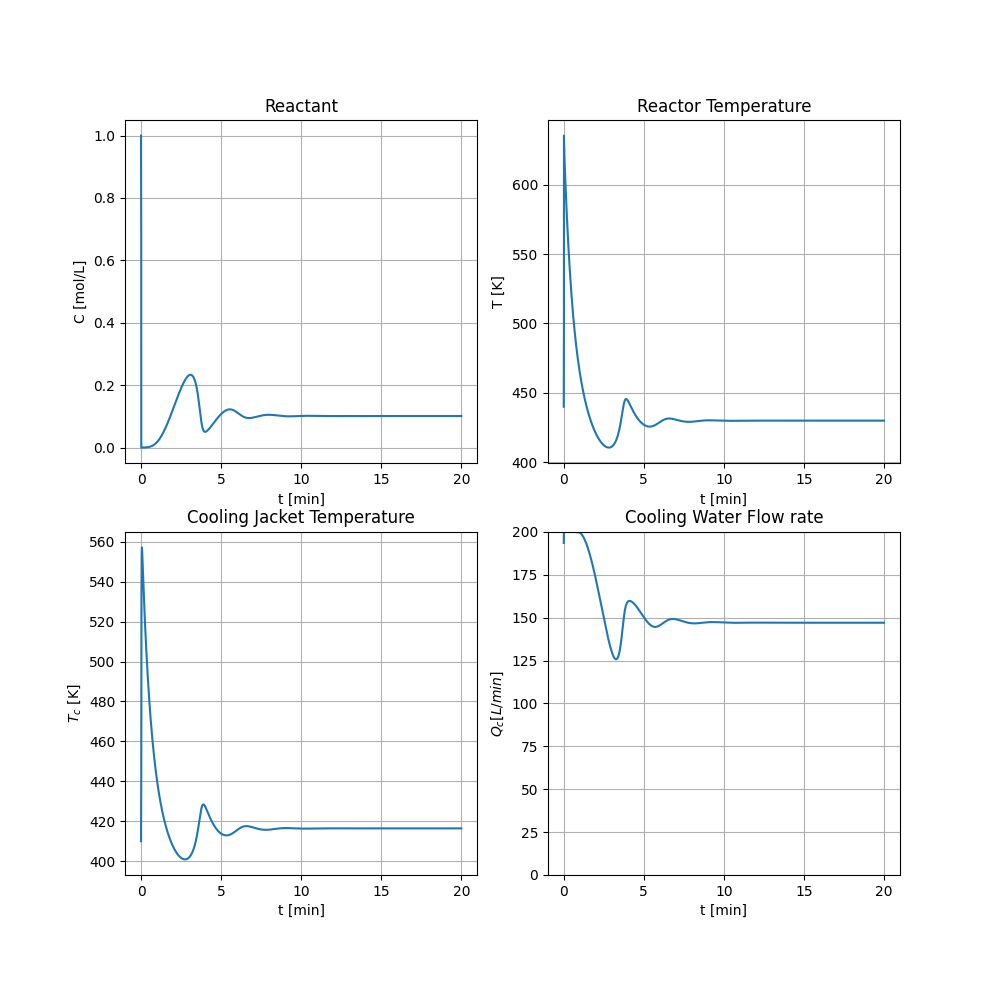
\includegraphics[width=1\textwidth]{img/baseline_model_results}
	\caption{System variables over time}
	\label{fig:baseline_model_results.png}
\end{figure}

The inlet conditions of the model were changed as detailed in Table \ref{tab:inlet_conditions} to analyse its sensitivity. The final values for each variable at different inlet conditions is shown in Table \ref{tab:baseline_model_sens}. As expected, there is little change in the concentration or the temperatures. However there is a more marked change in the final cooling water flow rate value. However the drop in $Q_c$ to 100 L/min could not be reproduced for the initial conditions at 120 minutes. This could be potentially due to the difference in controller parameters or a misunderstanding of the inlet conditions that were used. Therefore, the replicated model is clearly not exact.

\begin{table}[H]
	\caption{Inlet conditions at 0, 60, 120 and 180 mins}
	\label{tab:baseline_model_sens}
	\centering
\begin{tabular}{lrrrr}
	\toprule
	{} &    C &      T &   $T_c$ &   $Q_c$ \\
	\midrule
	0 mins   &  0.1 &  430.0 &  416.39 &  147.01 \\
	60 mins  &  0.1 &  430.0 &  416.31 &  144.12 \\
	120 mins &  0.1 &  430.0 &  416.44 &  139.36 \\
	180 mins &  0.1 &  430.0 &  417.87 &  124.70 \\
	\bottomrule
\end{tabular}
\end{table}

\subsection{Dataset Generation: Substandard Operation}

The model presented in Section \ref{sec:substandard} was simulated with the varying inlet conditions given in Figure \ref{fig:dataset_substandard_inlet} below for a sample 1200 minutes. The step changes in the inlet conditions can be seen to occur every 60 minutes. 

\begin{figure}[H]
	\centering
	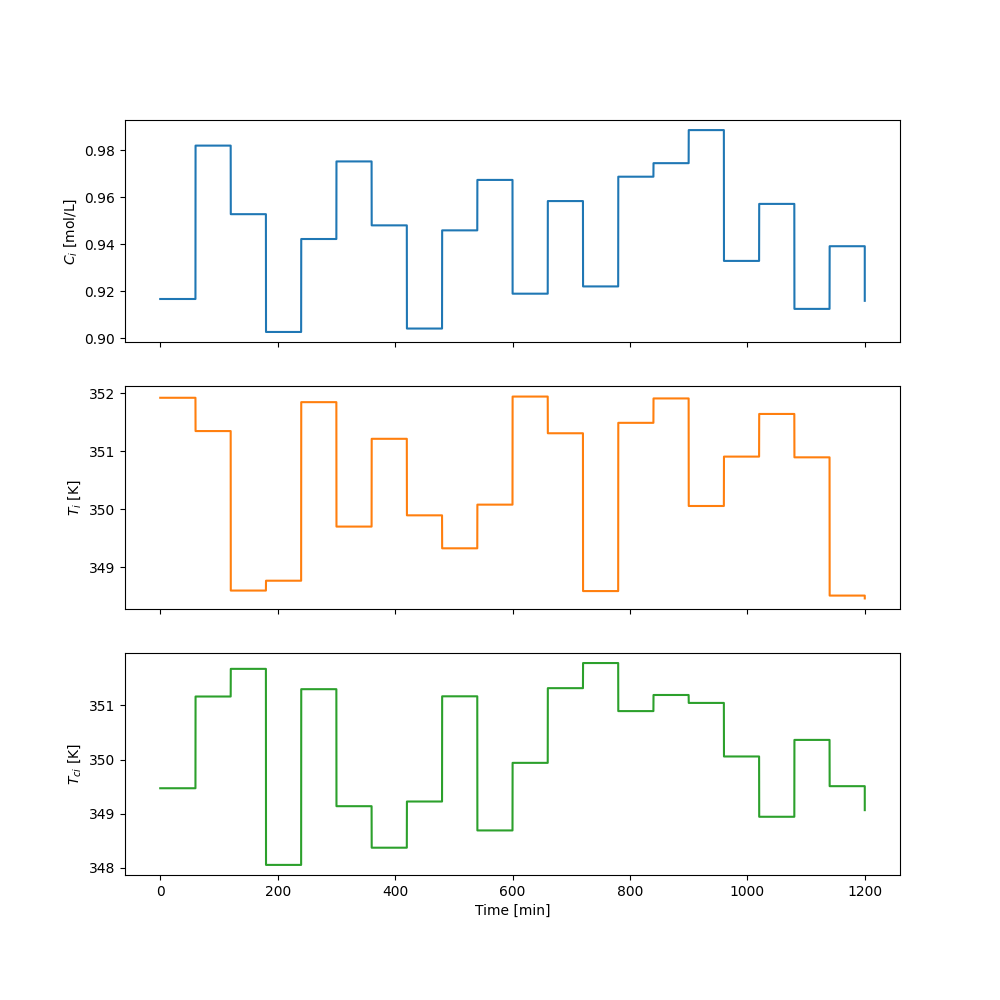
\includegraphics[width=1\textwidth]{img/dataset_substandard_inlet}
	\caption{Inlet conditions over time for simulation}
	\label{fig:dataset_substandard_inlet}
\end{figure}


The results of this run are shown in Figure \ref{fig:dataset_substandard_sample}. The perturbations in the inlet conditions can be seen to cause step changes in the dynamic variables with the exception of the reactor temperature which is maintained at its setpoint of 430 K. A noticeable increasing trend can be seen in the cooling water flowrate indicating that the system is having a harder time at controlling the temperature. This is coupled with a decreasing trend in the cooling jacket temperature which is due to the fouling of the jacket leading to a lower heat transfer capability. Another noticeable trend is in the reactant concentration which is increasing. This is due to the decay of the catalyst which is causing less reactant to be converted over time. The large spikes in the values are due to solver errors when conditions are abruptly changed. This is somewhat indicative of real data where spikes in sensor readings can happen due to abrupt process changes. 

\begin{figure}[H]
	\centering
	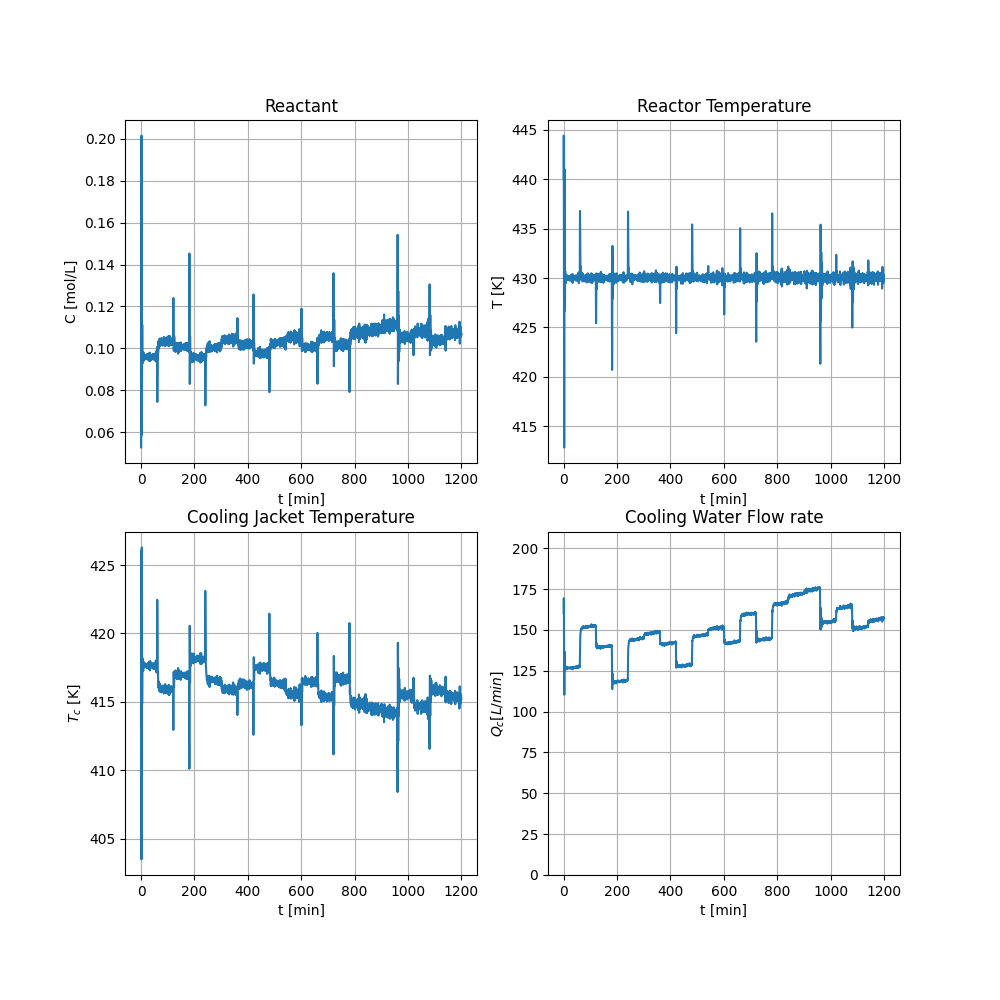
\includegraphics[width=1\textwidth]{img/dataset_substandard}
	\caption{System variables over time for substandard model}
	\label{fig:dataset_substandard_sample}
\end{figure}

As a final measure of obfuscating the data, we add Gaussian noise to all dynamic sensor values and shift some of the variables to replicate sensor drift. This gives a full set of results as shown in Figure \ref{fig:dataset_substandard_all_sample} below. 

\begin{figure}[H]
	\centering
	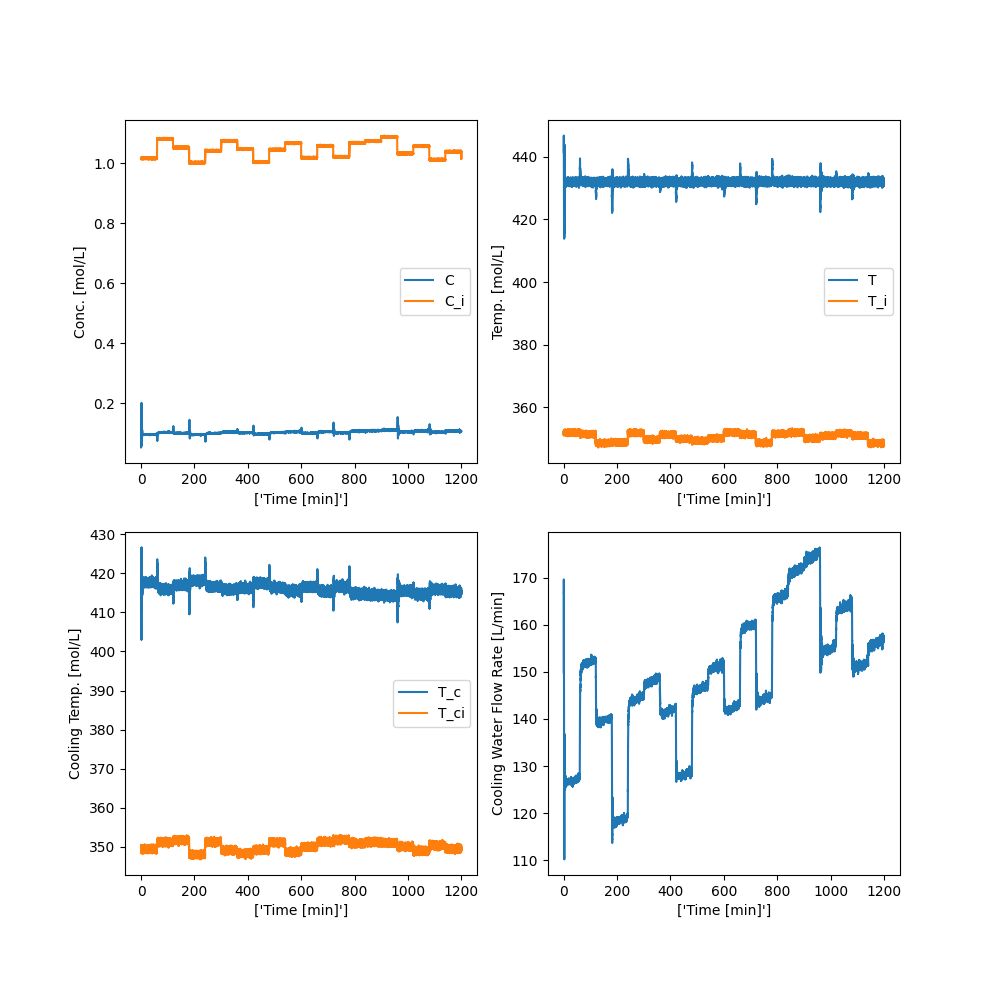
\includegraphics[width=1\textwidth]{img/dataset_substandard_all_sample}
	\caption{All system variables over time for substandard model after drift and noise}
	\label{fig:dataset_substandard_all_sample}
\end{figure}



\section{Conclusion}

Model is somewhat replicated with the exception of the controller parameters and the drop in the flowrate for certain inlet conditions. It's possible that the inlet conditions mentioned weren't used to generate those results or that the controller behaviour is fundamentally different. The code is stable and can be freely used by anyone to generate a data set for further research and analysis.


\bibliography{cstr_model}

\end{document}